% Options for packages loaded elsewhere
\PassOptionsToPackage{unicode}{hyperref}
\PassOptionsToPackage{hyphens}{url}
%
\documentclass[
]{article}
\usepackage{lmodern}
\usepackage{amssymb,amsmath}
\usepackage{ifxetex,ifluatex}
\ifnum 0\ifxetex 1\fi\ifluatex 1\fi=0 % if pdftex
  \usepackage[T1]{fontenc}
  \usepackage[utf8]{inputenc}
  \usepackage{textcomp} % provide euro and other symbols
\else % if luatex or xetex
  \usepackage{unicode-math}
  \defaultfontfeatures{Scale=MatchLowercase}
  \defaultfontfeatures[\rmfamily]{Ligatures=TeX,Scale=1}
\fi
% Use upquote if available, for straight quotes in verbatim environments
\IfFileExists{upquote.sty}{\usepackage{upquote}}{}
\IfFileExists{microtype.sty}{% use microtype if available
  \usepackage[]{microtype}
  \UseMicrotypeSet[protrusion]{basicmath} % disable protrusion for tt fonts
}{}
\makeatletter
\@ifundefined{KOMAClassName}{% if non-KOMA class
  \IfFileExists{parskip.sty}{%
    \usepackage{parskip}
  }{% else
    \setlength{\parindent}{0pt}
    \setlength{\parskip}{6pt plus 2pt minus 1pt}}
}{% if KOMA class
  \KOMAoptions{parskip=half}}
\makeatother
\usepackage{xcolor}
\IfFileExists{xurl.sty}{\usepackage{xurl}}{} % add URL line breaks if available
\IfFileExists{bookmark.sty}{\usepackage{bookmark}}{\usepackage{hyperref}}
\hypersetup{
  hidelinks,
  pdfcreator={LaTeX via pandoc}}
\urlstyle{same} % disable monospaced font for URLs
\usepackage{graphicx}
\makeatletter
\def\maxwidth{\ifdim\Gin@nat@width>\linewidth\linewidth\else\Gin@nat@width\fi}
\def\maxheight{\ifdim\Gin@nat@height>\textheight\textheight\else\Gin@nat@height\fi}
\makeatother
% Scale images if necessary, so that they will not overflow the page
% margins by default, and it is still possible to overwrite the defaults
% using explicit options in \includegraphics[width, height, ...]{}
\setkeys{Gin}{width=\maxwidth,height=\maxheight,keepaspectratio}
% Set default figure placement to htbp
\makeatletter
\def\fps@figure{htbp}
\makeatother
\setlength{\emergencystretch}{3em} % prevent overfull lines
\providecommand{\tightlist}{%
  \setlength{\itemsep}{0pt}\setlength{\parskip}{0pt}}
\setcounter{secnumdepth}{-\maxdimen} % remove section numbering

\title{4D Namespaces: Coxeter.4D, Einstein.4D, Fuller.4D}
\author{Daniel Ari Friedman\\ ORCID: 0000-0001-6232-9096\\ Email: daniel@activeinference.institute}
\date{August 14, 2025}

\begin{document}
\maketitle

\hypertarget{d-namespaces-coxeter.4d-einstein.4d-fuller.4d}{%
\section{4D Namespaces: Coxeter.4D, Einstein.4D,
Fuller.4D}\label{d-namespaces-coxeter.4d-einstein.4d-fuller.4d}}

In this section, we clarify the three internal meanings of ``4D,''
following a dot-notation that avoids cross-domain confusion. First we
briefly review the Coxeter.4D and Einstein.4D name spaces, which should
be familiar to most readers. We then review and highlight the Fuller.4D
name space, which is the focus of this manuscript.

\hypertarget{coxeter.4d-euclidean-eux2074}{%
\subsection{Coxeter.4D (Euclidean
E⁴)}\label{coxeter.4d-euclidean-eux2074}}

\begin{itemize}
\tightlist
\item
  \textbf{Definition}: standard E⁴ with orthogonal axes and Euclidean
  metric; the proper setting for classical regular polytopes. As Coxeter
  notes (Regular Polytopes, Dover ed., p.~119), this Euclidean 4D is not
  spacetime. Lattice/packing discussions connect to Conway \& Sloane's
  systematic treatment of higher-dimensional sphere packings and
  lattices
  (\href{https://link.springer.com/book/10.1007/978-1-4757-6568-7}{Sphere
  Packings, Lattices and Groups (Springer)}).
\item
  \textbf{Usage}: embed Quadray configurations or compare alternative
  parameterizations when a strictly Euclidean 4D setting is desired.
\item
  \textbf{Simplexes}: simplex structures extend naturally to 4D and
  beyond (e.g., pentachora).
\end{itemize}

\hypertarget{einstein.4d-relativistic-spacetime}{%
\subsection{Einstein.4D (Relativistic
spacetime)}\label{einstein.4d-relativistic-spacetime}}

\begin{itemize}
\item
  \textbf{Spacetime}: Minkowski metric signature.
\item
  \textbf{Line element} (mostly-plus convention; see
  \href{https://en.wikipedia.org/wiki/Minkowski_space}{Minkowski
  space}):

  \begin{equation}\label{eq:einstein_line_element}
  ds^2 = -c^2\,dt^2 + dx^2 + dy^2 + dz^2
  \end{equation}
\item
  \textbf{Optimization analogy}: metric-aware geodesics generalize to
  information geometry where the Fisher metric replaces the physical
  metric. See
  \href{https://en.wikipedia.org/wiki/Fisher_information}{Fisher
  information} and
  \href{https://en.wikipedia.org/wiki/Natural_gradient}{natural
  gradient}.
\end{itemize}

\hypertarget{fuller.4d-synergetics-quadrays}{%
\subsection{Fuller.4D (Synergetics /
Quadrays)}\label{fuller.4d-synergetics-quadrays}}

\begin{itemize}
\tightlist
\item
  \textbf{Basis}: four non-negative components A,B,C,D with at least one
  zero post-normalization, treated as a vector (direction and
  magnitude), not merely a point. Overview:
  \href{https://en.wikipedia.org/wiki/Quadray_coordinates}{Quadray
  coordinates}.
\item
  \textbf{Geometry}: tetrahedral; unit tetrahedron volume = 1; integer
  lattice aligns with close-packed spheres (IVM). Background:
  \href{https://en.wikipedia.org/wiki/Synergetics_(Fuller)}{Synergetics}.
\item
  \textbf{Distances}: computed via appropriate projective normalization;
  edges align with tetrahedral axes. The IVM = CCP = FCC shortcut allows
  working in 3D embeddings for visualization while preserving the
  underlying Fuller.4D tetrahedral accounting.
\item
  \textbf{Implementation heritage}: Extensive computational validation
  through Kirby Urner's
  \href{https://github.com/4dsolutions}{4dsolutions ecosystem},
  particularly
  \href{https://github.com/4dsolutions/m4w/blob/main/qrays.py}{\texttt{qrays.py}
  (vector operations)} and educational materials in
  \href{https://github.com/4dsolutions/School_of_Tomorrow}{School\_of\_Tomorrow}.
\end{itemize}

\hypertarget{directions-not-dimensions-language-and-models}{%
\subsubsection{Directions, not dimensions (language and
models)}\label{directions-not-dimensions-language-and-models}}

\begin{itemize}
\tightlist
\item
  \textbf{Vector-first framing}: Treat Quadrays as four canonical
  directions (``spokes'' to the vertices of a regular tetrahedron from
  its center), not as four orthogonal dimensions. The methane molecule
  (CH₄) and caltrop shape are helpful mental models.
\item
  \textbf{Origins outside Synergetics}: Quadrays did not originate with
  Fuller; we adopt the coordinate system within the IVM context. See
  \href{https://en.wikipedia.org/wiki/Quadray_coordinates}{Quadray
  coordinates}.
\item
  \textbf{Language games}: Quadrays and Cartesian are parallel vector
  languages on the same Euclidean container; teaching them together
  avoids oscillating between ``points now, vectors later.''
\end{itemize}

\hypertarget{figures}{%
\subsubsection{Figures}\label{figures}}

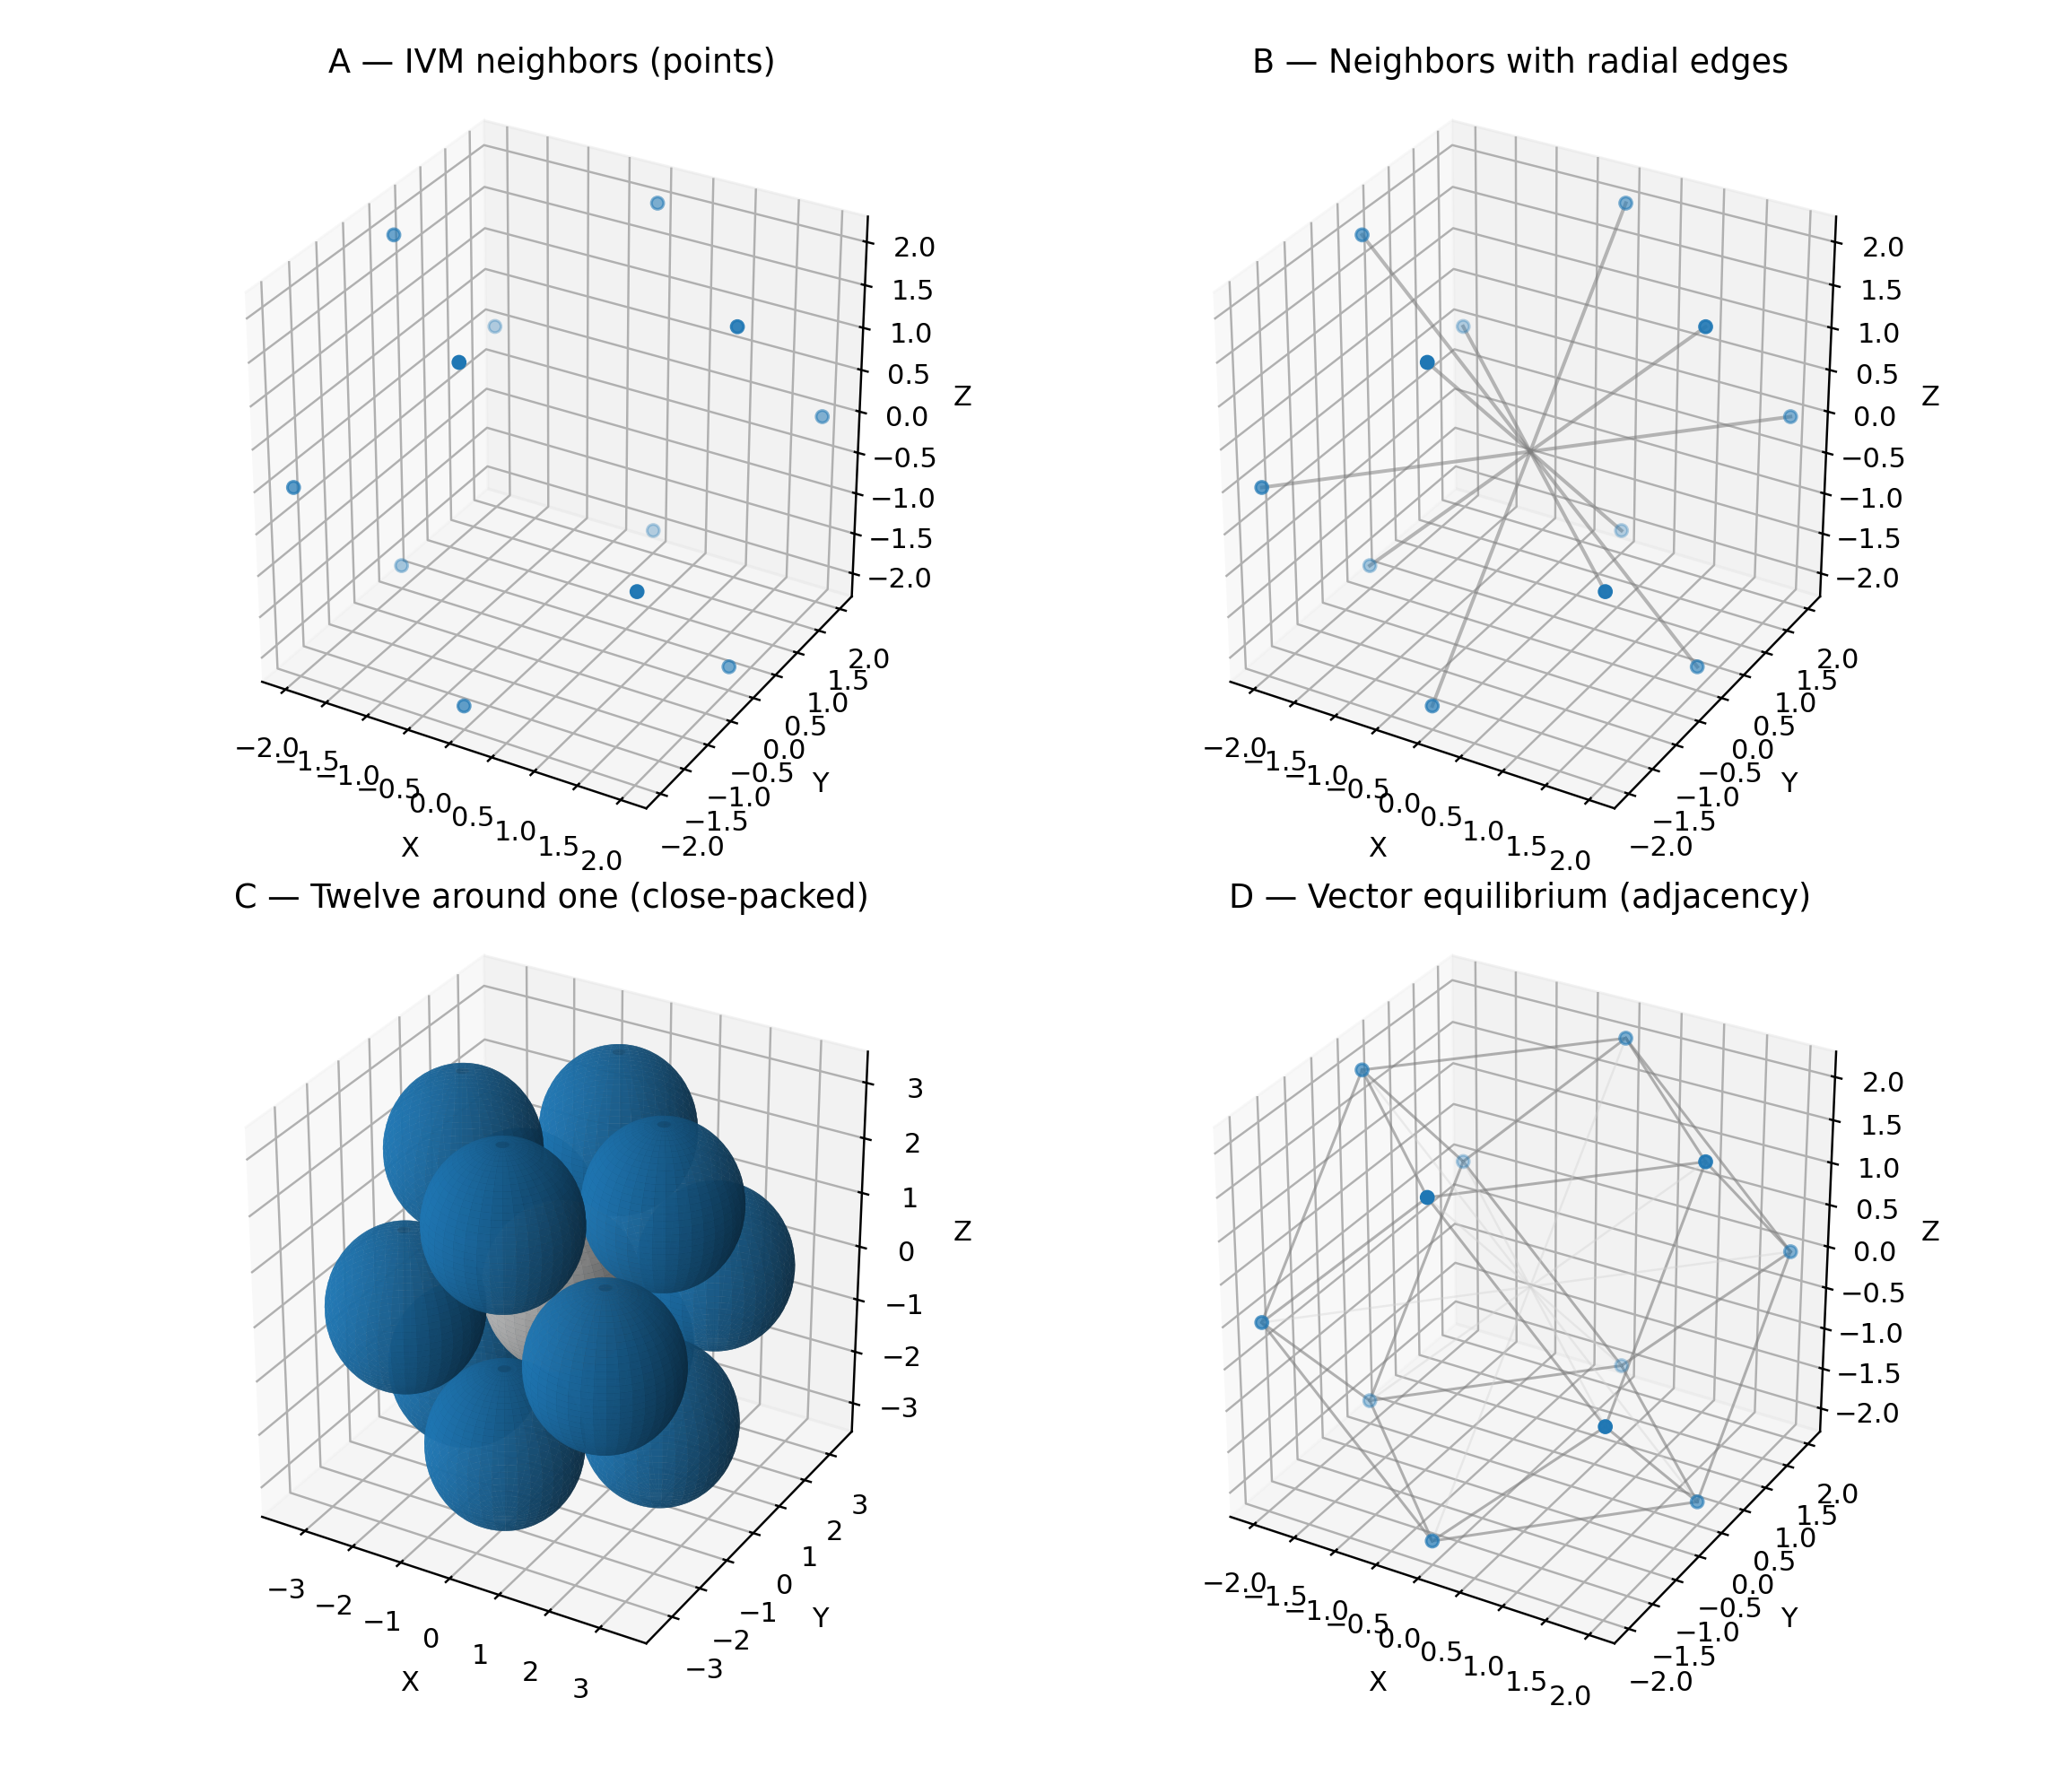
\includegraphics{../output/figures/ivm_neighbors_edges.png}
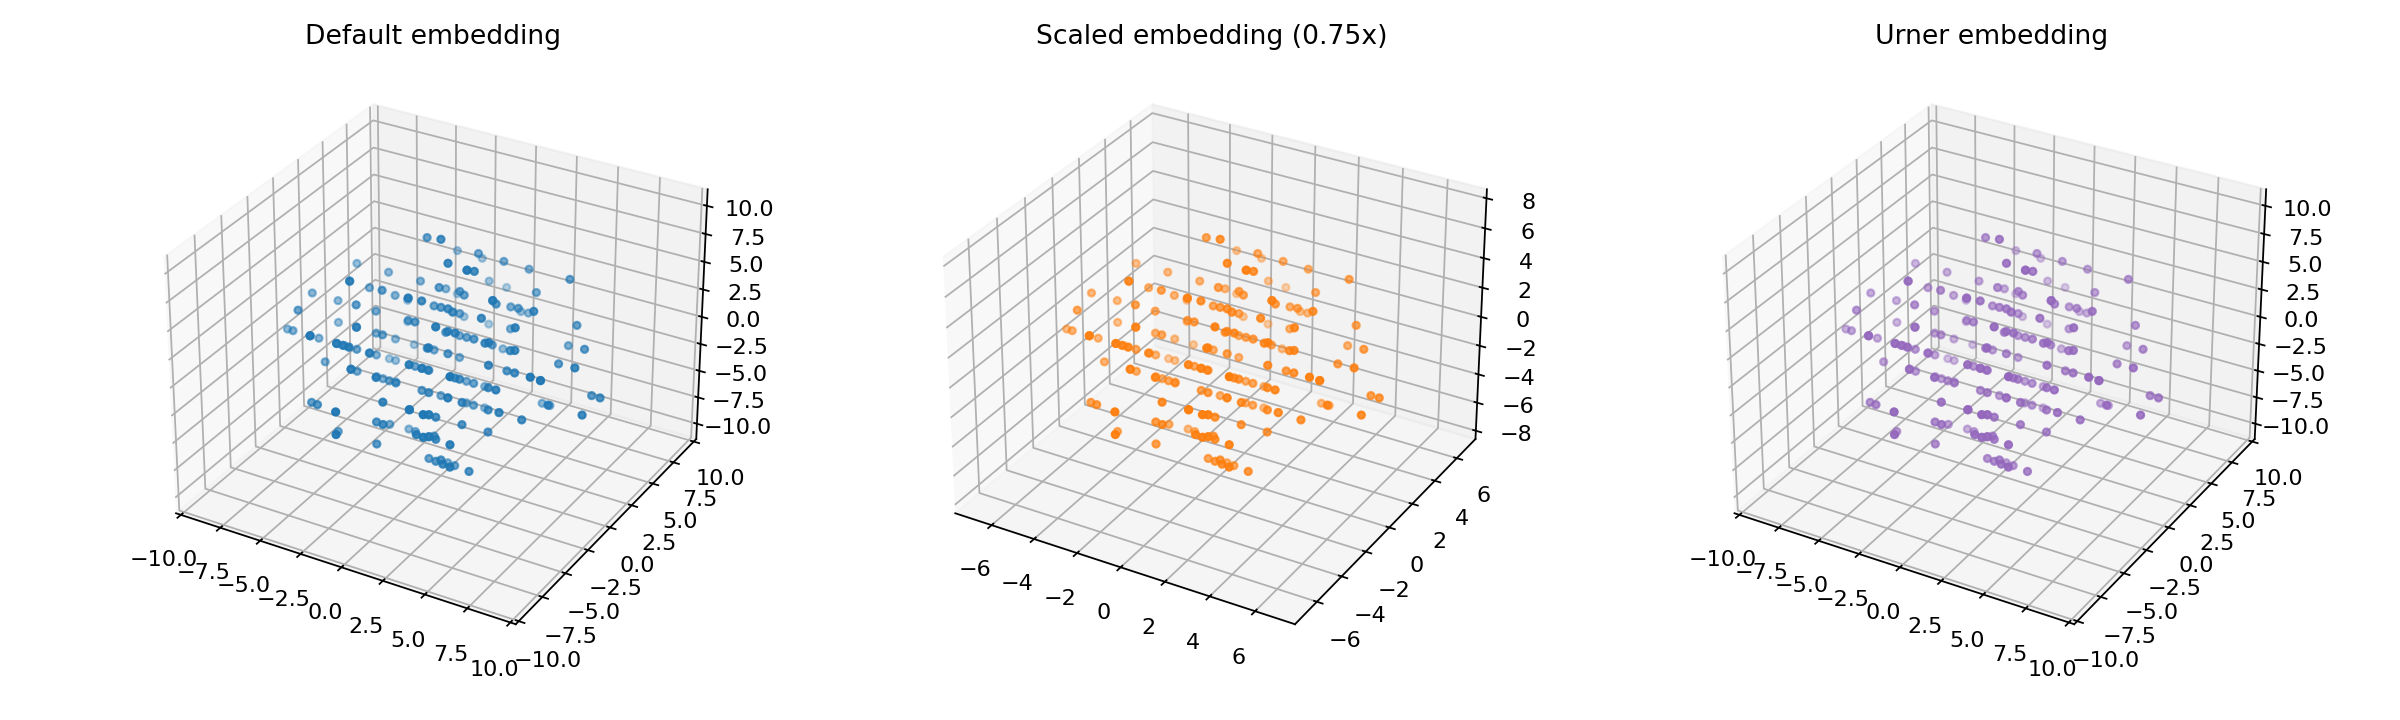
\includegraphics{../output/figures/quadray_clouds.png}
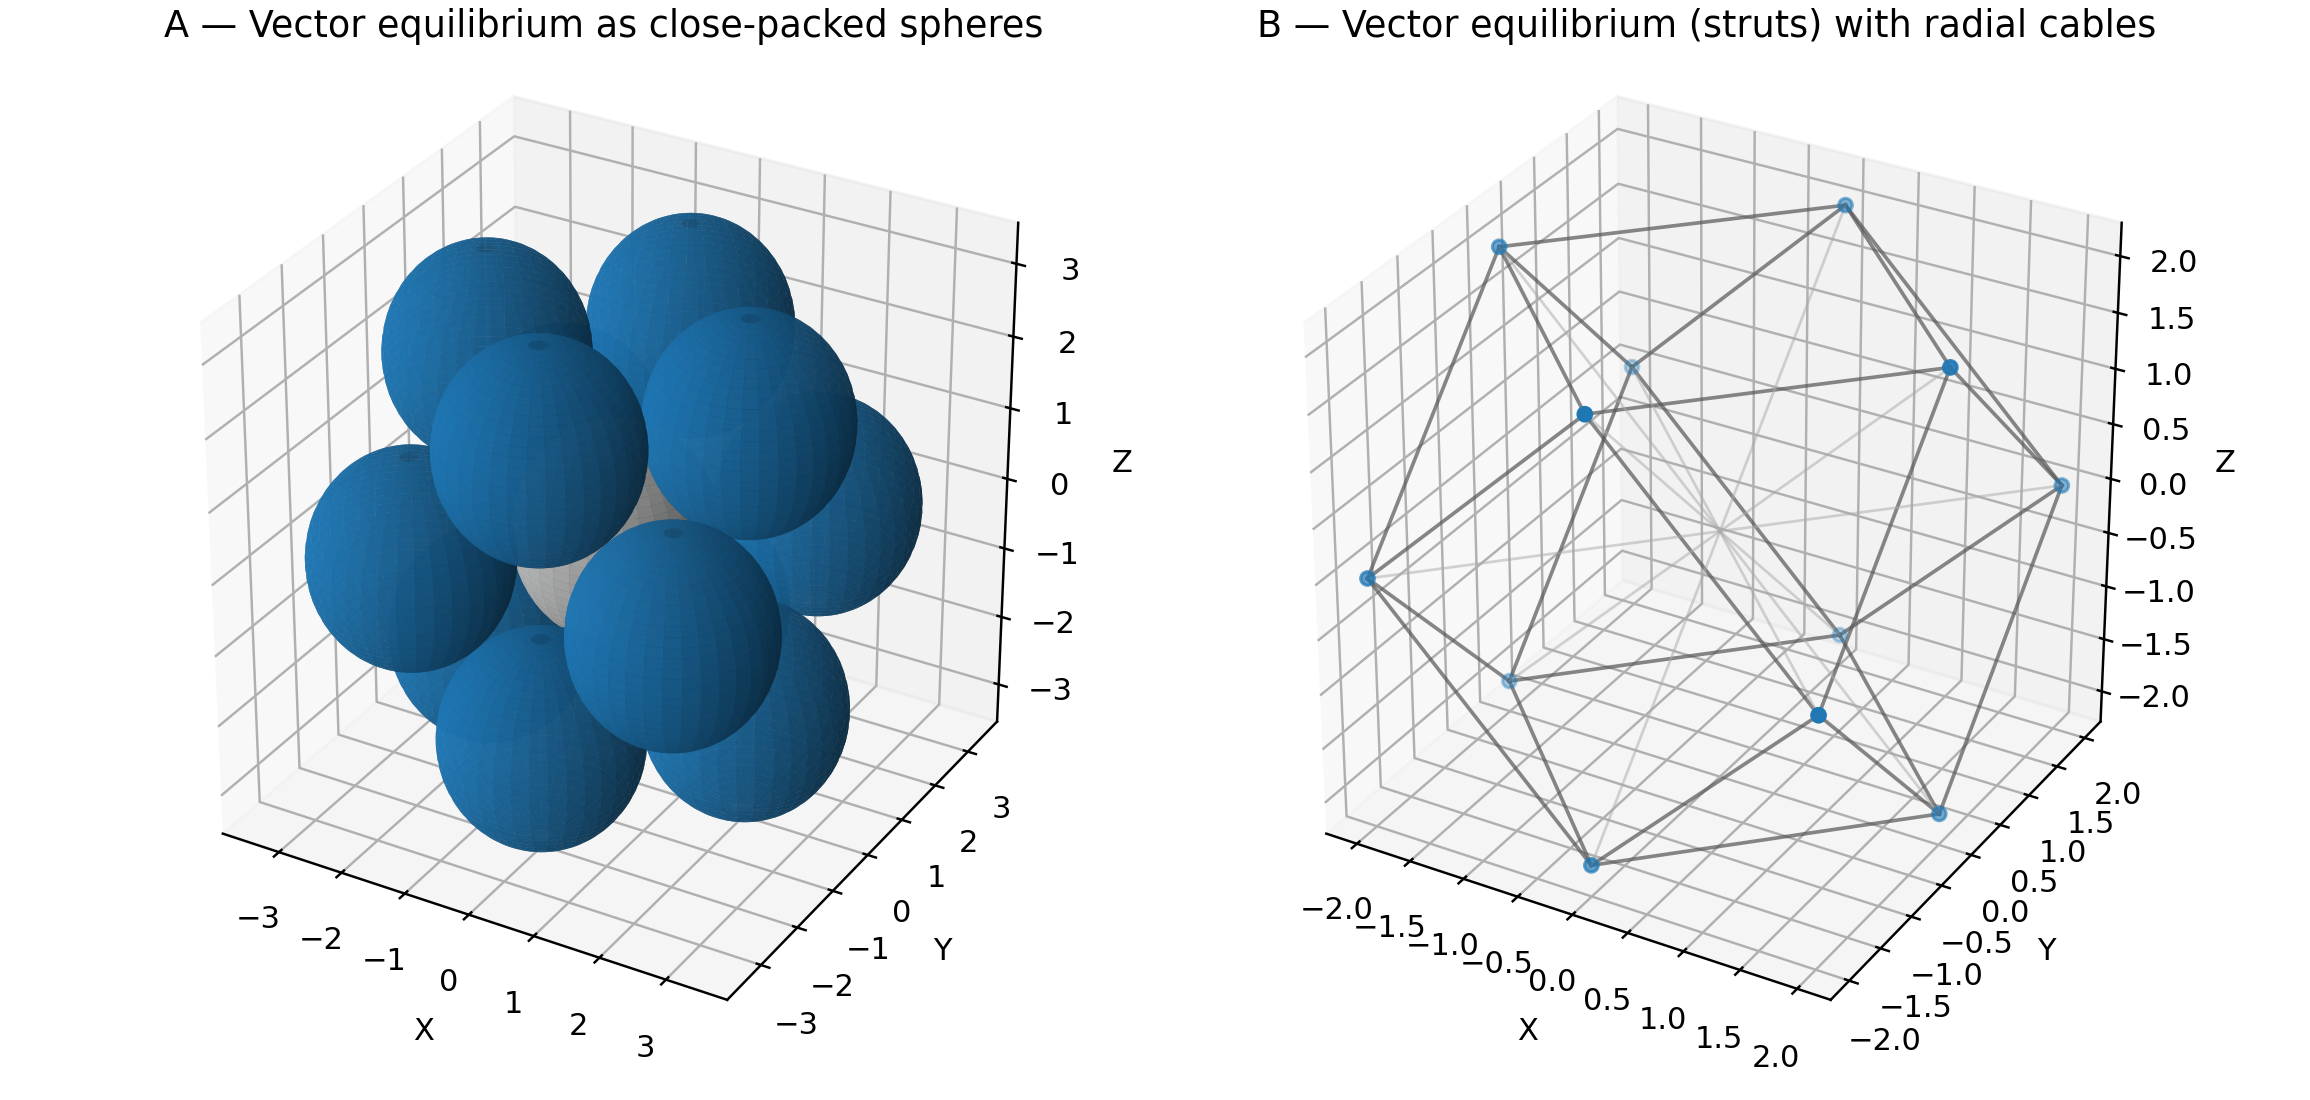
\includegraphics{../output/figures/vector_equilibrium_panels.png}

In Fig. \ref{fig:ivm_neighbors_edges}, we show the twelve nearest IVM
neighbors with radial edges under a standard Urner embedding; Fig.
\ref{fig:quadray_clouds} illustrates random Quadray clouds under several
embeddings.

Vector equilibrium (cuboctahedron). The shell formed by the 12 nearest
IVM neighbors is the cuboctahedron, also called the vector equilibrium
in synergetics. All 12 vertices are equidistant from the origin with
equal edge lengths, modeling a balanced local packing. This geometry
underlies the ``twelve around one'' close-packing motif and appears in
tensegrity discussions as a canonical balanced structure. See
background:
\href{https://en.wikipedia.org/wiki/Cuboctahedron}{Cuboctahedron (vector
equilibrium)} and synergetics references. Computational demonstrations
include
\href{https://github.com/4dsolutions/School_of_Tomorrow/blob/master/quadcraft.py}{\texttt{ivm\_neighbors.py}}
and related visualizations in the 4dsolutions ecosystem.

\hypertarget{clarifying-remarks}{%
\subsubsection{Clarifying remarks}\label{clarifying-remarks}}

\begin{itemize}
\tightlist
\item
  ``A time machine is not a tesseract.'' The tesseract is a Euclidean 4D
  object (Coxeter.4D), while Minkowski spacetime (Einstein.4D) is
  indefinite and not Euclidean; conflating the two leads to category
  errors. Fuller.4D, in turn, is a tetrahedral, mereological framing of
  ordinary space emphasizing shape/angle relations and IVM quantization.
  Each namespace carries distinct assumptions and should be used
  accordingly in analysis.
\end{itemize}

\hypertarget{practical-usage-guide}{%
\subsection{Practical usage guide}\label{practical-usage-guide}}

\begin{itemize}
\tightlist
\item
  Use \textbf{Fuller.4D} when working with Quadrays, integer
  tetravolumes, and IVM neighbors (native lattice calculations).
\item
  Use \textbf{Coxeter.4D} for Euclidean length-based formulas,
  higher-dimensional polytopes, or comparisons in E⁴ (including
  Cayley--Menger).
\item
  Use \textbf{Einstein.4D} as a metric analogy when discussing geodesics
  or time-evolution; do not mix with synergetic unit conventions.
\end{itemize}

\end{document}
